
\documentclass[12pt]{exam}
\usepackage{amsthm}
\usepackage{libertine}
%\usepackage[utf8]{inputenc}
\usepackage[margin=1in]{geometry}
\usepackage{amsmath,amssymb}
\usepackage{multicol}
\usepackage[shortlabels]{enumitem}
\usepackage{siunitx}
\usepackage{cancel}
\usepackage{graphicx}
\graphicspath{{./}}
\usepackage{pgfplots}
\usepackage{hyperref}
\usepackage{listings}
\usepackage{tikz}
\usepackage{minted}
\def\code#1{\texttt{#1}}
\usepackage{amssymb}
\usepackage{xcolor}
% for plotting
\usepackage{pgfplots}
\pgfplotsset{compat=1.16}
\usepackage{tikz}
\usetikzlibrary{arrows.meta}

\newcommand{\quotebox}[1]
{
  \begin{center}
    \fcolorbox{white}{blue!15!gray!15}{
      \begin{minipage}{0.7\linewidth}\vspace{10pt}
        \center
        \begin{minipage}{0.8\linewidth}{\space\Huge``}{\setlength{\parindent}{1.5em}#1}{\hspace{1.5em}\break\null\Huge\hfill''}
        \end{minipage}
        \smallbreak
      \end{minipage}
    }
\end{center}
}


% for plotting half circle
% call it with \MyHalfCircle{<size>}{<x coord>}{<y coord>} in tikz pictur
\newcommand{\MyHalfCircle}[3][0.4ex]{%
    % #1 = size
    % #2 = x coordinate
    % #3 = y coordinate
  \begin{scope}
   \draw (axis cs:#2,#3) circle (#1);
   \clip (axis cs:#2,#3) circle (#1);
   \fill[red, opacity=0.75] (axis cs:#2,#1) rectangle (axis cs:-#1,-#1);
  \end{scope}
}





%\DeclareUnicodeCharacter{2212}{-}



\let\oldemptyset\emptyset
\let\emptyset\varnothing

\hypersetup{
    colorlinks=true,
    linkcolor=blue,
    filecolor=magenta,      
    urlcolor=cyan,
    pdftitle={Overleaf Example},
    pdfpagemode=FullScreen,
    }
    
\urlstyle{same}

\pgfplotsset{width=10cm,compat=1.9}
\usepgfplotslibrary{external}
\tikzexternalize

\newcommand{\class}{Math 415} % This is the name of the course 
\newcommand{\examnum}{Homework-4} % This is the name of the assignment
\newcommand{\examdate}{Oct 11} % This is the due date
\newcommand{\timelimit}{}

\newcommand{\BO}{\mathcal{O}}




\begin{document}
\pagestyle{plain}
\thispagestyle{empty}

\noindent
\begin{tabular*}{\textwidth}{l @{\extracolsep{\fill}} r @{\extracolsep{6pt}} l}
\textbf{\class} & \textbf{Name:} & \textit{Zhenzhao Tu}\\ %Your name here instead, obviously 
\textbf{\examnum} &&\\
\textbf{\examdate} &&\\
\end{tabular*}\\
\rule[2ex]{\textwidth}{2pt}
% --


\section*{Problem 1}
The ODE
\[x'=h+rx-x^2\]
\begin{enumerate}[(a)]
	\item The bifurcation diagram $x$ vs. $r$ is shown below:
		\begin{enumerate}[(i)]
			\item For $h=0$, we have $x'=rx-x^2$. 
				
				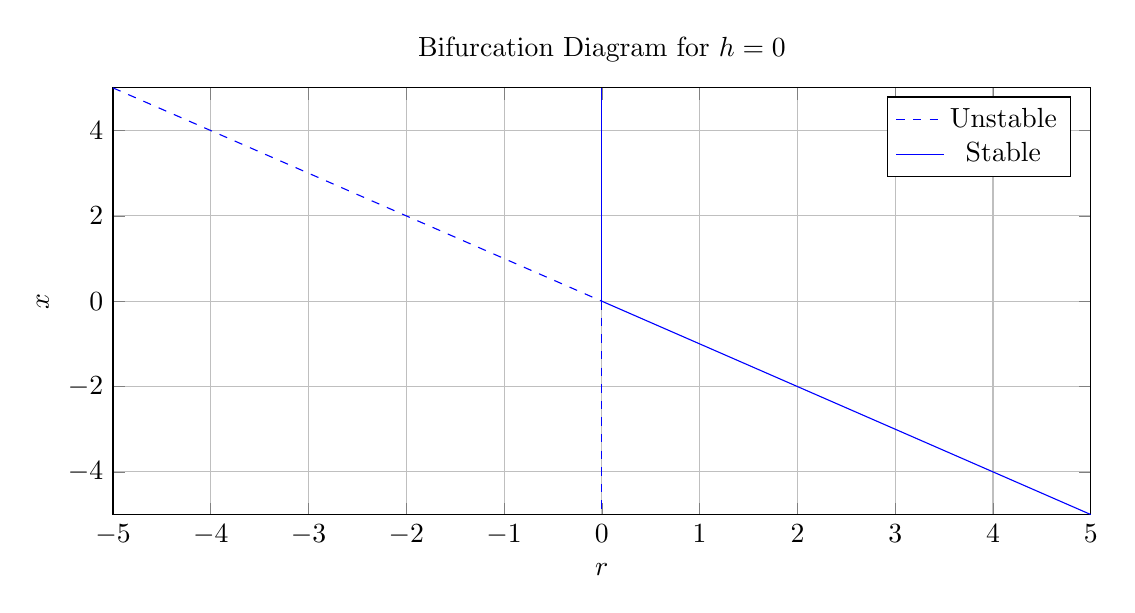
\begin{tikzpicture}
				\begin{axis}[
					title={Bifurcation Diagram for $h=0$},
					xlabel={$r$},
					ylabel={$x$},
					xmin=-5, xmax=5,
					ymin=-5, ymax=5,
					grid=major,
					width=14cm,
					height=7cm,
					]

					% -x where x < 0 with dashed line
					\addplot[blue, domain=-5:0, samples=100, dashed] {-x};
					% -x where x > 0 with line
					\addplot[blue, domain=0:5, samples=100] {-x};
					% add vertical line at y = 0 from x = 0 to x = 5
					\addplot[blue, domain=0:5, samples=100] coordinates {(0, 0) (0, 5)};
					% add vertical dashed line at y = 0 from x = 0 to x = -5
					\addplot[blue, domain=-5:0, samples=100, dashed] coordinates {(0, 0) (0, -5)};

				
				\legend{Unstable, Stable}
				\end{axis}
				
				\end{tikzpicture}

			\item For $h<0$, we have $x'=-4+rx-x^2$. 
				
				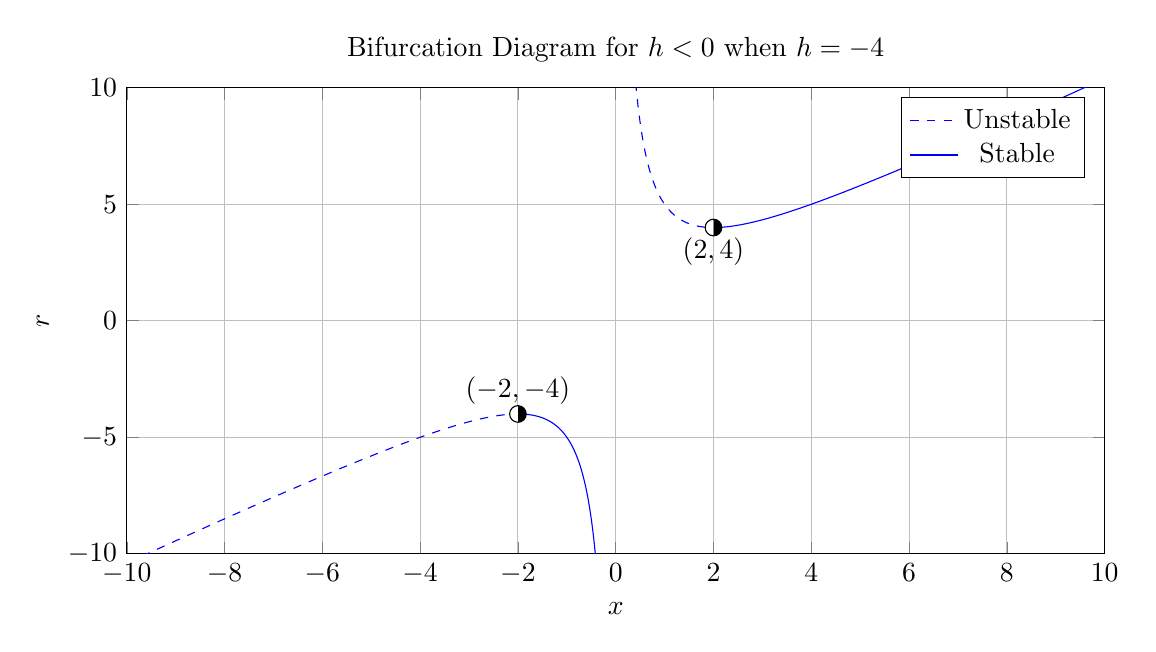
\begin{tikzpicture}
				\begin{axis}[
					title={Bifurcation Diagram for $h<0$ when $h=-4$},
					xlabel={$x$},
					ylabel={$r$},
					xmin=-10, xmax=10,
					ymin=-10, ymax=10,
					grid=major,
					width=14cm,
					height=7.5cm,
					]

					% (x^2+4)/x where x < -2 with dashed line
					\addplot[blue, domain=-10:-2, samples=100, dashed] {(x^2+4)/x};
					% (x^2+4)/x where x > -2 and x < 0 with line
					\addplot[blue, domain=-2:-0.01, samples=100] {(x^2+4)/x};
					% (x^2+4)/x where x > 0 and x < 2 with dashed line
					\addplot[blue, domain=0.01:2, samples=100, dashed] {(x^2+4)/x};
					% (x^2+4)/x where x > 2 with line
					\addplot[blue, domain=2:10, samples=100] {(x^2+4)/x};

					% add half point at (-2, -4)
					\addplot[mark=halfcircle*, mark options={rotate=-90}, mark size=3pt] coordinates {(-2, -4)} node[above]{$(-2,-4)$};
					% add half point at (2, 4)
					\addplot[mark=halfcircle*, mark options={rotate=-90}, mark size=3pt] coordinates {(2, 4)} node[below]{$(2,4)$};
				
				\legend{Unstable, Stable}
				\end{axis}
				
				\end{tikzpicture}

			\item For $h>0$, we have $x'=4+rx-x^2$.
				
				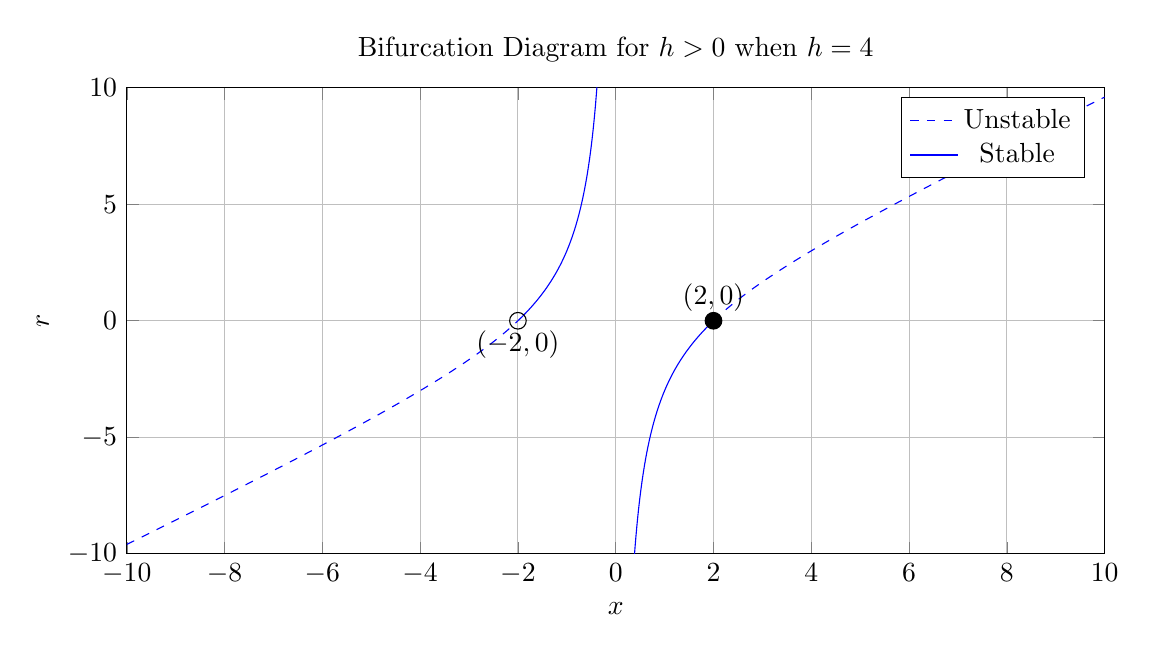
\begin{tikzpicture}
				\begin{axis}[
					title={Bifurcation Diagram for $h>0$ when $h=4$},
					xlabel={$x$},
					ylabel={$r$},
					xmin=-10, xmax=10,
					ymin=-10, ymax=10,
					grid=major,
					width=14cm,
					height=7.5cm,
					]

					% (x^2-4)/x where x < -2 with dashed line
					\addplot[blue, domain=-10:-2, samples=100, dashed] {(x^2-4)/x};
					% (x^2-4)/x where x > -2 and x < 0 with line
					\addplot[blue, domain=-2:-0.01, samples=100] {(x^2-4)/x};
					% (x^2-4)/x where x > 0 and x < 2 with line
					\addplot[blue, domain=0.01:2, samples=100] {(x^2-4)/x};
					% (x^2-4)/x where x > 2 with dashed line
					\addplot[blue, domain=2:10, samples=100, dashed] {(x^2-4)/x};

					% add hollow point at (-2, 0)
					\addplot[only marks, mark=o, mark size=3pt] coordinates {(-2, 0)} node[below]{$(-2,0)$};
					% add point at (2, 0)
					\addplot[only marks, mark=*, mark size=3pt] coordinates {(2, 0)} node[above]{$(2,0)$};
				
				\legend{Unstable, Stable}
				\end{axis}
				
				\end{tikzpicture}

			
		\end{enumerate}

	\item The the regions in the $(r, h)$-planeis can be calculated as $x^2=h+rx$. By taking derivative both sides of equation. We have $2x=r$, then plugin back to $x^2=h+rx$ we have
		\[ h=-x^2, \quad r=2x. \]
		We can use discriminant to find the region. The discriminant is $4h+r^2$.

		Then the plot is shown below:

		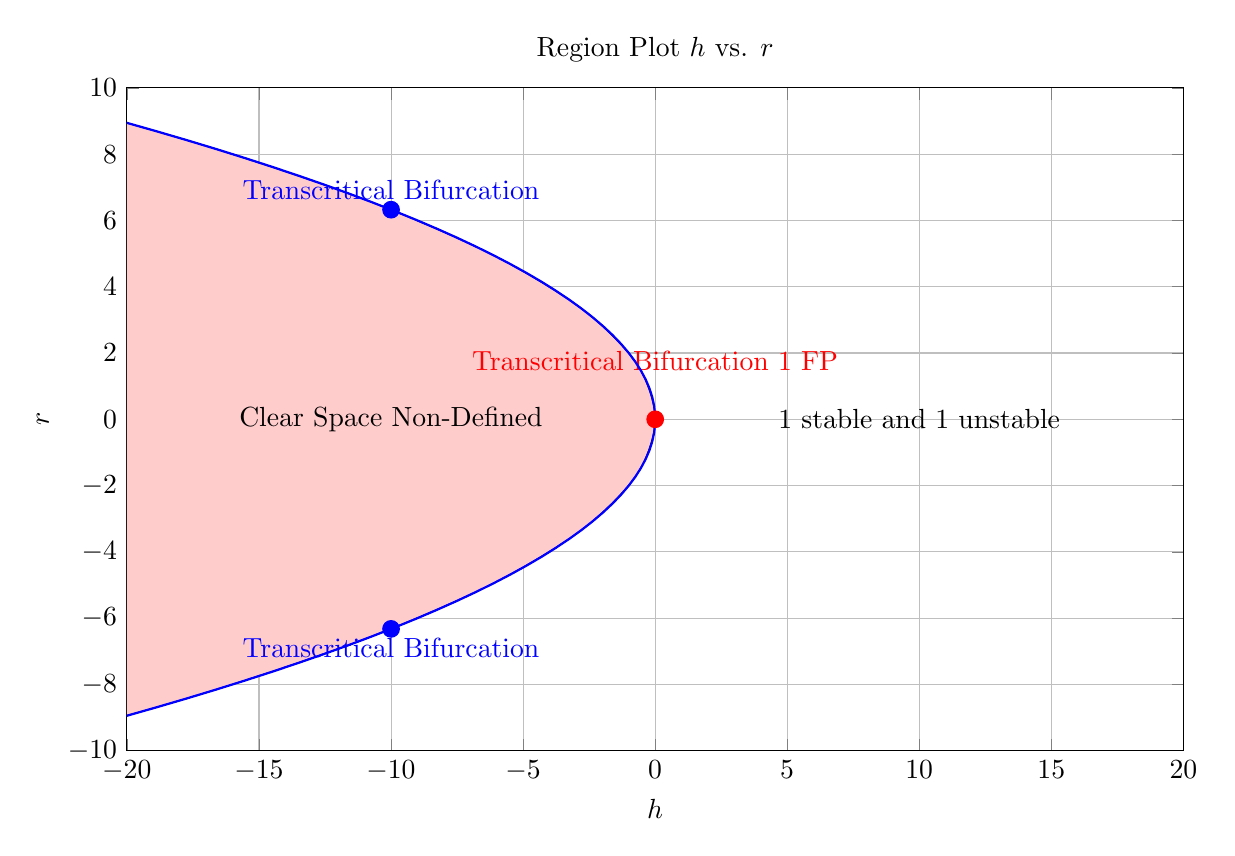
\begin{tikzpicture}
		\begin{axis}[
			title={Region Plot $h$ vs. $r$},
			xlabel={$h$},
			ylabel={$r$},
			xmin=-20, xmax=20,
			ymin=-10, ymax=10,
			grid=major,
			width=15cm,
			height=10cm,
			]

			% \sqrt(4x) from -20 to 20 by parametric equations
			\addplot[blue, domain=-20:20, samples=300, variable=\x] plot ({-\x*\x}, {2*\x});
			% fill red region -0.25x^2 from -20 to 20
			\addplot [fill=red!20, domain=-20:20] [smooth] ({-0.25*x*x}, x) -- cycle;
			% add text at (-10, 0) for the red region
			\node at (axis cs:-10,0) {Clear Space Non-Defined};
			% add text at (10, 0) for the blue region
			\node at (axis cs:10,0) {$1$ stable and $1$ unstable};
			% add point at (0, 0) 
			\addplot[only marks, mark=*, mark size=3pt, red] coordinates {(0, 0)} node[above, yshift=5mm]{Transcritical Bifurcation $1$ FP};
			
			% \sqrt(-4x) from -20 to 20
			\addplot[blue, thick, domain=-20:20, samples=300, variable=\x] plot ({-\x*\x}, {-2*\x});
			% add blue point at (-10, \sqrt(40))
			\addplot[only marks, mark=*, mark size=3pt, blue] coordinates {(-10, 6.324)} node[above]{Transcritical Bifurcation};
			% add blue point at (-10, -\sqrt(40))
			\addplot[only marks, mark=*, mark size=3pt, blue] coordinates {(-10, -6.324)} node[below]{Transcritical Bifurcation};
		


		\end{axis}
		\end{tikzpicture}


\end{enumerate}

\section*{Problem 2}
The IVP
\[\epsilon x''+x'+x=0, \quad x(0)=1, \quad x'(0)=0\]

\begin{enumerate}
	\item For analytically solution, we can use charateristic equation to solve it. The characteristic equation is
		\[\epsilon r^2+r+1=0.\]
		Then the roots are
		\[r_{1,2}=\frac{-1\pm\sqrt{1-4\epsilon}}{2\epsilon}.\]
		Given that $\epsilon>0$, then we consider
		\[x(t)= c_1e^{r_1t}+c_2e^{r_2t}.\]
		Using initial condition $x(0)=1$ and $x'(0)=0$, we have
		\[c_1 = \frac{-4\epsilon+\sqrt{1-4\epsilon}+1}{2-8\epsilon}, \quad c_2 = \frac{4\epsilon+\sqrt{1-4\epsilon}-1}{2+8\epsilon}.\]
		Then the solution is
		\[x(t)=\frac{-4\epsilon+\sqrt{1-4\epsilon}+1}{2-8\epsilon}e^{-\frac{\sqrt{1-4\epsilon }+1}{2\epsilon}t}+\frac{4\epsilon+\sqrt{1-4\epsilon}-1}{2+8\epsilon}e^{\frac{-1+\sqrt{1-4\epsilon}}{2\epsilon} t}.\]

	\item For $\epsilon \ll 1$, we know that the presence of the $\epsilon$ term will make the solution decay faster while the lower terms $x', x$ will change slower. Therefore, there are two dominant timescales $t_1$ and $t_2$ associated with fast and slow dynamics, respectively.
		In characteristic equation, we have $r_{1,2}$ in part (1), so let's analyze the roots.
		\[r_{1,2}=\frac{-1\pm\sqrt{1-4\epsilon}}{2\epsilon}.\]
		When $\epsilon \ll 1$, and by given $\sqrt{1-4\epsilon}\approx 1-2\epsilon+\BO(\epsilon^2)$, we have
		\[r_2= \frac{-1+\sqrt{1-4\epsilon}}{2\epsilon} \approx \frac{-1+1-2\epsilon}{2\epsilon} = -1.\]
		and
		\[r_1= \frac{-1-\sqrt{1-4\epsilon}}{2\epsilon} \approx \frac{-1-1+2\epsilon}{2\epsilon} = \frac{\epsilon-1}{\epsilon} = 1-\frac{1}{\epsilon}.\]
		Then we have $r_1=-1$ the root remains of the order of $1$ as $\epsilon \to 0$, and $r_2=1-\frac{1}{\epsilon}$ the root becomes large as $\epsilon \to 0$. Therefore, we have $r_1$ is the slow timescale and $r_2$ is the fast timescale.
		Thus, the two timescales $\tau_1$ and $\tau_2$ are
		\[\tau_2 = \frac{1}{|r_2|} = 1, \quad \tau_1 = \frac{1}{|r_1|} = \frac{1}{|1-\frac{1}{\epsilon}|} = \frac{\epsilon}{1-\epsilon}.\]
		
	\item Now let's plot the $x(t)$ and with two timescales $\tau_2=1, \tau_1=\frac{\epsilon}{1-\epsilon}$. Then we can plot the solution for $\epsilon=0.1$ as shown below:
			
				\begin{figure}[H]
					\centering
					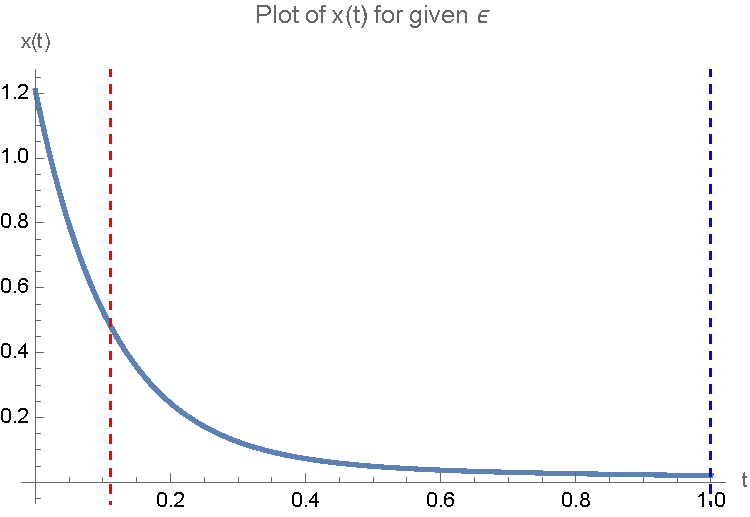
\includegraphics[width=0.8\linewidth] {x(t).pdf}
					\caption{Solution for $\epsilon=0.1$, Red line is $\tau_2$ and blue line is $\tau_1$.}
					
				\end{figure}

	\item When is valid to replace $\epsilon x''+x'+x=0$ with singular limit $x'+x=0$. 
					Let's consider the singular limit $x'+x=0$, then we know that it is also $x(t) = c_1e^{-t}$. If we looking back to the solution in part (1), we know that to such singular limit, we have to set $c_2\exp(t-t/\epsilon)=0$. However, only $t \to \infty$ can make $c_2\exp(t-t/\epsilon)=0$. Therefore, the statement is valid when $t$ is significantly large to infinity.

\end{enumerate}


\section*{Problem 3}
Consider two-dimensional system
\[x'=-y, \quad y'=-x.\]

\begin{enumerate}
	\item First we find the matrix $A$ for this system. The $\mathbf{x}'=A\mathbf{x}$, then we have
		\[\begin{bmatrix} x' \\ y' \end{bmatrix} = \begin{bmatrix} 0 & -1 \\ -1 & 0 \end{bmatrix} \begin{bmatrix} x \\ y \end{bmatrix}.\]
		Then the eigenvalues are
		\[\lambda_1 = -1, \quad \lambda_2 = 1.\]
		Then the eigenvectors are
		\[\mathbf{v}_1 = \begin{bmatrix} 1 \\ 1 \end{bmatrix}, \quad \mathbf{v}_2 = \begin{bmatrix} -1 \\ 1 \end{bmatrix}.\]
		Then the general solution is
		\[x(t) = c_1e^{-t}+c_2e^t, \quad y(t) = c_1e^{-t}-c_2e^t.\]

		\newpage
		Now, let's plot the vector field for it:

		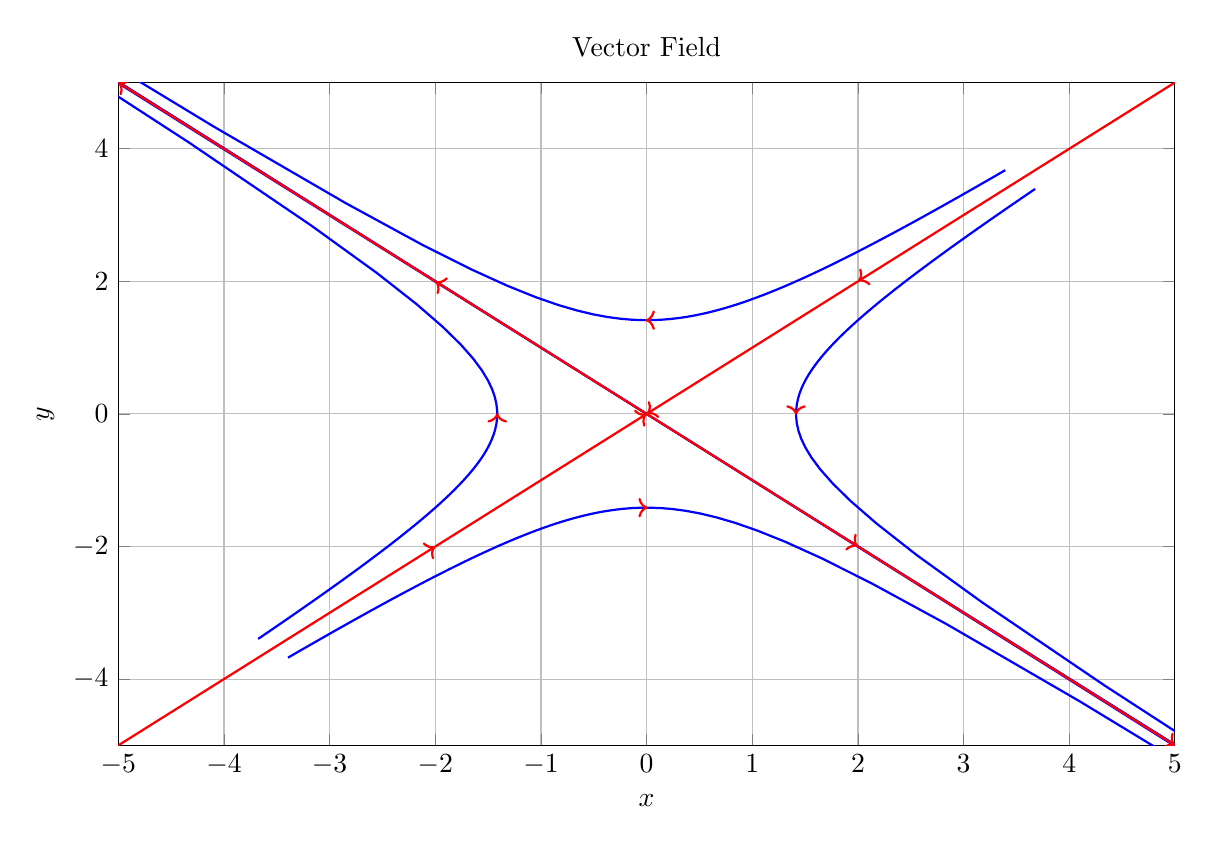
\begin{tikzpicture}
		\begin{axis}[
			title={Vector Field},
			xlabel={$x$},
			ylabel={$y$},
			xmin=-5, xmax=5,
			ymin=-5, ymax=5,
			grid=major,
			width=15cm,
			height=10cm,
			]

			% x from -5 to 5
			\addplot[blue, domain=-5:5, samples=100, variable=\x] plot ({\x}, {-\x});
			% -x from -5 to 5
			\addplot[blue, domain=-5:5, samples=100, variable=\x] plot ({\x}, {\x});
			% 1/x rotate -45 degree from -5 to 5
			\addplot[blue, thick, variable=\t, domain=-5:5, samples=150] ({t*sqrt(2)/2 - 1/t*sqrt(2)/2}, {t*sqrt(2)/2 + 1/t*sqrt(2)/2});
			% 1/x rotate +45 degree from -5 to 5
			\addplot[blue, thick, variable=\t, domain=-5:5, samples=150] ({t*sqrt(2)/2 + 1/t*sqrt(2)/2}, {t*sqrt(2)/2 - 1/t*sqrt(2)/2});

			% add vector from (5,5) to (2,2)
			\addplot[->, red, thick] coordinates {(5, 5) (2, 2)};
			% add vector from (2,2) to (0,0)
			\addplot[->, red, thick] coordinates {(2, 2) (0, 0)};
			% add vector from (-5,-5) to (-2,-2)
			\addplot[->, red, thick] coordinates {(-5, -5) (-2, -2)};
			% add vector from (-2,-2) to (0,0)
			\addplot[->, red, thick] coordinates {(-2, -2) (0, 0)};
			% add vector from (0, 0) to (-2, 2)
			\addplot[->, red, thick] coordinates {(0, 0) (-2, 2)};
			% add vector from (-2, 2) to (-5, 5)
			\addplot[->, red, thick] coordinates {(-2, 2) (-5, 5)};
			% add vector from (0, 0) to (2, -2)
			\addplot[->, red, thick] coordinates {(0, 0) (2, -2)};
			% add vector from (2, -2) to (5, -5)
			\addplot[->, red, thick] coordinates {(2, -2) (5, -5)};

			% add vector from (-1.414, -0.01) to (-1.414, 0.01)
			\addplot[->, red, thick] coordinates {(-1.414, -0.01) (-1.414, 0.01)};
			% add vector from (1.414, 0.01) to (1.414, -0.01)
			\addplot[->, red, thick] coordinates {(1.414, 0.01) (1.414, -0.01)};
			% add vector from (0.01, 1.414) to (-0.01, 1.414)
			\addplot[->, red, thick] coordinates {(0.01, 1.414) (-0.01, 1.414)};
			% add vector from (-0.01, -1.414) to (0.01, -1.414)
			\addplot[->, red, thick] coordinates {(-0.01, -1.414) (0.01, -1.414)};



		\end{axis}
		\end{tikzpicture}
		
	\item Consider $xx', yy'$, since $x'=-y, y'=-x$, we have
		\[xx' = -xy, \quad yy' = -yx.\]
		Then we have
		\[xx'-yy' = 0.\]
		Now integrate both sides of the equation, we have	
		\begin{align*}
			\int xx'-yy' \, dt &= \int 0 \, dt \\
			\int xx' \, dt - \int yy' \, dt &= 0 \\
			\int x \, dx - \int y \, dy &= 0 \\
			\frac{1}{2}x^2 - \frac{1}{2}y^2 &= c \\
			x^2 - y^2 &= C.
		\end{align*}
		Then we have $x^2-y^2=C$ is the invariant manifold.
		

	\item As we showed in the graph. The $x$ is unstable manifold and $y$ is stable manifold. Then the invariant manifold is the line $x^2-y^2=C$.

\end{enumerate}


\section*{Problem 4}
Consider the epidemic model
\[\begin{cases}
	x' = -kxy, \\
	y' = kxy-ly, \\
	z' = ly,
\end{cases}
\text{subject to} \quad 
\begin{cases}
	x(0) = x_0, \\
	y(0) = y_0, \\
	z(0) = 0.
\end{cases}\]

\begin{enumerate}
	\item When we add $x', y', z'$ togather, we have
		\[x'+y'+z' = -kxy+kxy-ly+ly = 0.\]
		Then ww integrate both sides of the equation, we have
		\begin{align*}
			\int x'+y'+z' \, dt &= \int 0 \, dt \\
			\int x' \, dt + \int y' \, dt + \int z' \, dt &= \int 0 \\
			x+y+z &= x_0+y_0 +0.
		\end{align*}
	
	\item Given $z'=ly$, rewrite as $y=z'/l$, then plugin to $x'=-kxy$, we have
		\[x'=-kx\frac{z'}{l}.\]
		Then we can solve $x$ by using separation of variables:
		\begin{align*}
			\frac{dx}{dt} &= -\frac{kx}{l}\frac{dz}{dt} \\
			\frac{dx}{x} &= -\frac{k}{l}dz \\
			\int \frac{dx}{x} &= -\frac{k}{l}\int dz \\
			x(t) &= x_0e^{-k\frac{z}{l}}.
		\end{align*}
		So we have $x(t)$ is a function of $z(t)$.

	\item Consider $z'=ly$, given $x+y+z=x_0+y_0$ from (1), we have
		\[z' = l(x_0+y_0-z-x).\]
		As we also showed from (2), $x(t) = x_0\exp(-kz/l)$, then we have
		\[z' = l(x_0+y_0-z-x_0\exp(-kz/l)).\]
		
	\item To do non-dimensionalization to this ODE, we first set
					\[u = \frac{k}{l}z, \quad \tau = \frac{x_0}{k}t.\]
		Then consider
		\[\frac{dz}{dt} = \frac{dz}{d\tau}\frac{d\tau}{dt} = \frac{dz}{d\tau}\frac{x_0}{k}.\]
		Then we have
		\[\frac{dz}{d\tau} = \frac{k}{x_0}\frac{dz}{dt}.\]
		Recall the ODE in (3), we have
		\begin{align*}
			\frac{du}{d\tau} &= \frac{1}{lx_0}\frac{dz}{dt} \\
					 &= \frac{l}{lx_0}(x_0+y_0-z-x_0 e^{-\frac{kz}{l}}) \\
			&= \frac{x_0+y_0}{x_0}-\frac{z}{x_0}-e^{-\frac{kz}{l}}) \\
			&= \frac{x_0+y_0}{x_0}-\frac{u}{x_0}-e^{-u}.
		\end{align*}
		Therefore, the $a$ and $b$ are	
		\[a = \frac{x_0+y_0}{x_0}, \quad b = \frac{1}{x_0}.\]
		
	\item As shown in (4), we have
		\[a=\frac{x_0+y_0}{x_0}, \quad b=\frac{1}{x_0}.\]
		Then we are going to analyze the range of $a$ and $b$.
	Since $x_0$ represents the initial number of healthy people and $y_0$ represents the initial number of infected people, they are both non-negative. Then we have $a=(x_0+y_0)/x_0=1+x_0/y_0 > 1$. Also, since $x_0 \geq 0$ but $b$ is not allow $x_0=0$, we have $b > 0$. Therefore, we show that $a>1$ and $b>0$.






\end{enumerate}







\end{document}

